\newpage
%%%%%%%%%%%%%%%%%%%%%%%%%%%%%%%%%%%%%%%%%%%%%%%%%%%%%%%%%%%%%%%%
%%%%%%%%%%%%%%%%%%%%%%%%%%%%%%%%%%%%%%%%%%%%%%%%%%%%%%%%%%%%%%%%
%%%%%%%%%%%%%%%%%%%%%%%%%% Enunciado %%%%%%%%%%%%%%%%%%%%%%%%%%%

\begin{myblock}
\phantomsection\addcontentsline{toc}{section}{Ejercicio \#3 | Análisis de Conteo de Parejas de Cangrejos Cacerola Mediante un GML Poisson}
\section*{Ejercicio \#3 | Análisis de Conteo de Parejas de Cangrejos Cacerola Mediante un GML Poisson}

Entre los cangrejos cacerola se sabe que cada hembra tiene un macho en su nido, pero puede tener más 
machos concubinos. Se considera que la variable respuesta es el número de concubinos y las variables
explicativas son: color, estado de la espina central, peso y anchura del caparazón.\\

\begin{center}
\begin{tabular}{ccccc}
\hline
\textbf{Color} & \textbf{Spine} & \textbf{Width} & \textbf{Satellite} & \textbf{Weight} \\
\hline
3 & 3 & 28.3 & 8 & 3050 \\
4 & 3 & 22.5 & 0 & 1550 \\
2 & 1 & 26.0 & 9 & 2300 \\
4 & 3 & 24.8 & 0 & 2100 \\
4 & 3 & 26.0 & 4 & 2600 \\
3 & 3 & 23.8 & 0 & 2100 \\
2 & 1 & 26.5 & 0 & 2350 \\
\hline
\end{tabular}
\end{center}

Realiza e interpreta los resultaados de ajustar un modelo lineal generalziado tipo Poisson. 

\end{myblock}

%%%%%%%%%%%%%%%%%%%%%%%%%%%%%%%%%%%%%%%%%%%%%%%%%%%%%%%%%%%%%%%%
%%%%%%%%%%%%%%%%%%%%%%%%%%%%%%%%%%%%%%%%%%%%%%%%%%%%%%%%%%%%%%%%

%%%%%%%%%%%%%%%%%%%%%%%%%%%%%%%%%%%%%%%%%%%%%%%%%%%%%%%%%%%%%%%%
%%%%%%%%%%%%%%%%%%%%%%%%%%%%%%%%%%%%%%%%%%%%%%%%%%%%%%%%%%%%%%%%

\subsection{Teoría}

En lo que respecta a Modelos Lineales Generalizados, el modelo Poisson constituye la herramienta
fundamental para analizar datos de conteo. En la pequeña base de datos que nos han otorgado, tenemos 
información sobre cangrejos cacelora, en la cual encontramos características físcias como el color, 
datos de la espina, anchura y peso. Estos datos fueron medidos de la hembra, es decir, se busca 
encontrar relación entre las características físicas de la hembra y la cantidad de concubinos que 
tiene. 

Este problema se compone de un avariable de respuesta $Y_i$, que es el número de concubinos (o machos satélite)
que acompañan a cada hembra. Tenemos un conteo de la siguiente forma:

\[
    Y_i \in \{0, 1, 2, ...., n\}
\]

Por ello, nuestro modelo a construir sera uno de Poisson, pues es el que mejor se acopla cuando tenemos 
una variable de interés con un conteo de eventos, tipo el número de clientes de una empresa, el número
de errores en un examen, o el número de miembros en un conjunto de animales. Recordemos que la distribución
Poisson con parámetro $\mu_i > 0$ tiene:

\[
    \text{P}(Y_i = y_i) = \frac{e^{-\mu_i} \mu_i^{y_i}}{y_i !} \;\;\;\;\; \text{con} \;\; y_i = 0,1,2,...
\]

En este caso, $\mu_i$ representa el número de concubinos de la cangrejo hembra. 

Ahora bien, en un GLM Poisson, tenemos la distribución de la familia exponencial $Y_i \sim \text{Poisson}(\mu_i)$. 
El enlace canico será:

\[
    g(\mu_i) = \log(\mu_i)
\]

Lo cual garantiza que $\mu_i > 0$. Así, el predictor lineal es:

\[
    \log(\mu_i) = \eta_i = \beta_0 + \beta_1 x_1 + \beta_2 x_2 + ...
\]

Finalmente, para nuestro caso, tenemos:

\[
    \log(\mu_i) = \beta_0 + \beta_1 \cdot \text{Color}_i + \beta_2 \cdot \text{Spine}_i + \beta_3 \cdot \text{Width}_i + \beta_4 \cdot \text{Weight}_i
\]

Podemos darle de inicio un poco de contexto sobre cómo se hará la interpretación. Bajo escala logarítmica,
tenemos:

\[
    \log(\mu_i) = \beta_0 + \beta_j x_{ij}
\] 

Exponenciando:

\[
    \mu_i = e^{\beta_0} \cdot e^{\beta_j x_{ij}}
\]

De ese modo, $e^{\beta_j}$ se interpreta como una razón de tasas de incidencia, o \textit{Incidence Rate Ratio} (IRR). Así:

\begin{itemize}
    \item Si $x_{ij}$ aumenta en una unidad, entonces $\mu_i$ se multiplica por $e^{\beta_j}$
    \item Si $e^{\beta_j} > 1$, entonces la variable incrementa el número esperado de concubinos.
    \item Si $e^{\beta_j} < 1$, entonces la variable reduce el número esperado de concubinos.
\end{itemize}

Por ejemplo, bajo este caso, suponiendo que tuvieramos un $\beta_3 = 0.25$. entonces $e^{0.25} \approx 1.28$
nos estaría diciendo que por cada aumento de una unidad en anchura, se espera un 28\% más de concubinos. Eso 
manteniendo las demás variables como constantes.

%%%%%%%%%%%%%%%%%%%%%%%%%%%%%%%%%%%%%%%%%%%%%%%%%%%%%%%%%%%%%%%%%%%%%%%%%%%
%%%%%%%%%%%%%%%%%%%%%%%%%%%%%%%%%%%%%%%%%%%%%%%%%%%%%%%%%%%%%%%%%%%%%%%%%%%

\subsection{Resultados}

\subsubsection{Anchura de Caparazón | \textit{Width}}

Para el caso de la varibale de anchura de caparazón, encontramos un IRR de 1.716 un un IC95\% de entre 1.28 y 2.29.
Es decir, por cada centímetro de anchura, se espera un incremento de concubinos del 71.6\%, o en otras
palabras, por cada centimetro, se multiplica el número de concubinos por 1.716 unidades. El Intercepto
tiene un valor de $2.16 \times 10^{-6}$. Entonces, podemos utilizar la media esperada para realizar predicciones,
esto se puede observar en el cuadro \ref{tab:width-capa}.\\

\begin{table}[h!]
    \centering
    \begin{tabular}{|c|c|}
        \hline
        \textbf{Anchura (cm)} & $\boldsymbol{\hat{\mu}}$ \textbf{(concubinos esperados)} \\
        \hline
        22.5 & 0.41 \\
        \hline
        24.0 & 0.92 \\
        \hline
        24.8 & 1.42 \\
        \hline
        26.0 & 2.71 \\
        \hline
        28.0 & 7.98 \\
        \hline
        28.3 & 9.38 \\
        \hline
    \end{tabular}
    \caption{Incremento de concubinos por cm.}
    \label{tab:width-capa}
\end{table}

Los resultados del cuadro anterior son consistentes con lo encontrado por la evidencia gráfica. La curvas
predicha nos indica que para anchiras pequeñas, de entre 22 y 24 centímetros, el valor esperado de
concubinos está entre 0 y 1. A partir de los 26 cm, la curva crece casi de manera exponencial,llegando a 
valores de 5 hasta 9 concubinos esperados. Podemos argumentar entonces que hembras más grandes
pueden esperar tener una mayor cantidad de concubinos. 

\begin{figure}[h!]
    \centering
    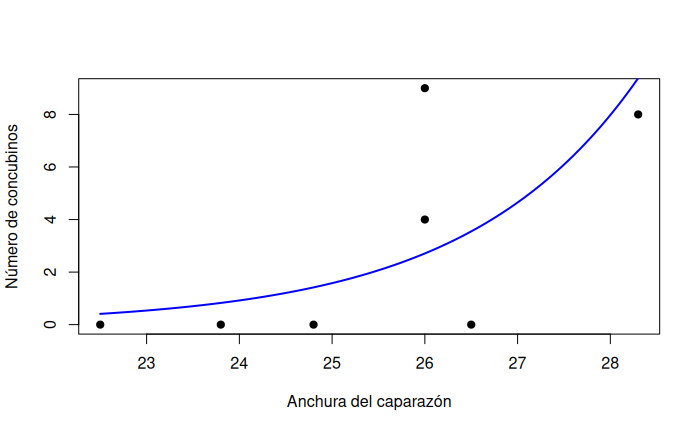
\includegraphics[width=0.7\linewidth]{Images/anchura-capa.png}
    \caption{Predicciones por anchura.}
    \label{fig:anchura-capa}
\end{figure}

Esto también es consistente con la biología de los cangrejos cacerola. Esta especie de animales presenta
dimorfismo sexual, es decir, hay una diferencia muy significativa entre el tamaño y la morfología de
los individuos hembra y macho. En el caso de los cangrejos cacerola, las hembras son mucho más grandes
que los machos, por lo que pueden ofrecer mayor protección y seguridad a una mayor cantidad de machos satélite.

Sin embargo, el crecimiento exponencial de concubinos seguramente debe tener un límite. Más datos serían
necesarios para comprender mejor cuál es la tendencia real. Aunque la evidencia es clara, mayor tamaño está
fuertemente correlacionado con mayor cantidad de concubinos. 

\subsubsection{Peso del Cangrejo | \textit{Weight}}

Para la variable peso, el modleo Poisson univariado arroja un IRR igual a 1.00194 por gramo, con IC95\%
entre 1.00088 y 1.00299. Es decir, por cada gramo adicional, el número de concubinos esperado se multiplica
por 1.00194. Quizás una lectura más práctica es que por cada 100 gramos, se espera un incrementro del
21.3\%.

El intercepto estimado es de 0.0253. Con este parámetro y la pendiente, podemo susar la media esperada $\hat{\mu}$
para hacer predicciones en pesos de interés, esto se resume como en el cuadro \ref{tab:peso-concubinos}.

\begin{table}[h!]
    \centering
    \begin{tabular}{|c|c|}
        \hline
        \textbf{Peso (g)} & \textbf{$\hat{\mu}$ (concubinos esperados)} \\
        \hline
        1550 & 0.51 \\
        \hline
        2100 & 1.46 \\
        \hline
        2350 & 2.37 \\
        \hline
        2600 & 3.85 \\
        \hline
        3050 & 9.19 \\
        \hline
    \end{tabular}
    \caption{Incremento de concubinos por peso}
    \label{tab:peso-concubinos}
\end{table}

Nuevamente, estos resultados son coherentes con la evidencia grfica: a bajos pesos, se esperan muy pocos 
concubinos, y al acercarnos a los 3,000 graos, la curva aumenta de forma marcada, alcanzando valores de
concubinos satélite de entre 4 y 9 miembros. Entonces, el peso también está fuertemente relacionado
con la cantidad de acompañantes de una hembra. Esto tiene mucho sentido, a mayor anchura, se puede 
esperar mayor peso, y a mayor peso mayor anchura.

\begin{figure}[h!]
    \centering
    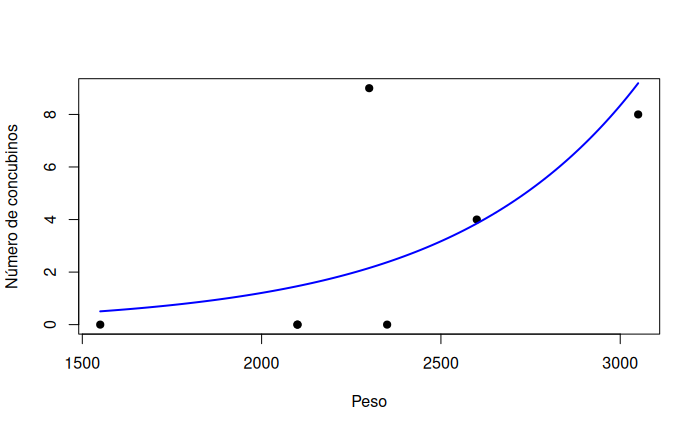
\includegraphics[width=0.7\linewidth]{Images/peso-capa.png}
    \caption{Predicciones por peso.}
    \label{fig:peso-capa}
\end{figure}

\subsubsection{Color del Caparazón | \textit{Color}}

Para la variable de color del caparazón, el modelo Poisson univariado arroja un IRR de 0.889 para el nivel
Color 3 respecto al nivel de referencia (Color 2), con un IC95\% entre 0.343 y 2.304. Esto indica que en
promedio, las hembras con coloración 3 presentan un 11\% menos concubinos que aquellas con coloración 2,
aunque el intervalo de confianza incluye el valor 1, por lo que no existe evidencia estadísticamente clara
de una diferencia entre estos grupos.

En el caso del nivel Color 4, el IRR estimado es de 0.296 con un IC95\% entre 0.091 y 0.962. Esto implica
que las hembras con coloración 4 tienen alrededor de un 70\% menos concubinos que las hembras con coloración 2.
En este caso, el límite superior del intervalo se encuentra por debajo de 1, lo que sugiere una posible
diferencia significativa, aunque debe tomarse con cautela debido al reducido tamaño muestral.

La media esperada $\hat{\mu}$ para cada nivel de color se resume en el cuadro \ref{tab:color-concubinos}.

\begin{table}[h!]
    \centering
    \begin{tabular}{|c|c|}
        \hline
        \textbf{Color} & \textbf{$\hat{\mu}$ (concubinos esperados)} \\
        \hline
        2 & 4.50 \\
        \hline
        3 & 4.00 \\
        \hline
        4 & 1.33 \\
        \hline
    \end{tabular}
    \caption{Número esperado de concubinos por nivel de color.}
    \label{tab:color-concubinos}
\end{table}

Estos resultados concuerdan con la evidencia gráfica: los colores 2 y 3 muestran medianas más altas, mientras
que el color 4 concentra valores bajos. Aunque los datos sugieren que la coloración puede estar asociada a
diferencias en el número de concubinos, la baja cantidad de observaciones por nivel impide una conclusión
firme.

\begin{figure}[h!]
    \centering
    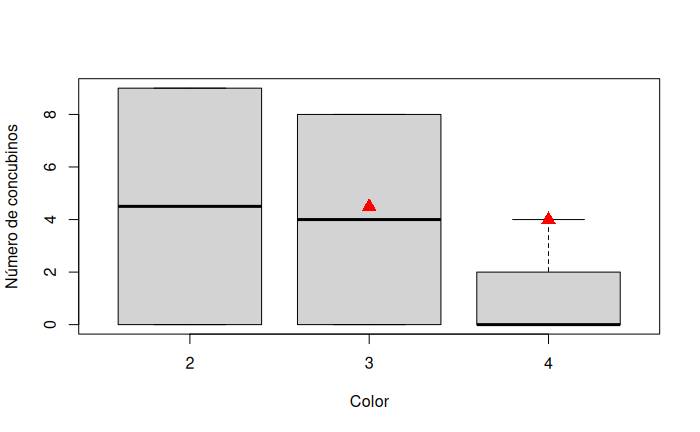
\includegraphics[width=0.7\linewidth]{Images/color-capa.png}
    \caption{Predicciones por color.}
    \label{fig:color-capa}
\end{figure}

\subsubsection{Estado de la Espina Central | \textit{Spine}}

Para la variable de estado de la espina central, el modelo Poisson univariado considera al nivel Spine 1
como referencia. El IRR estimado para Spine 3 es de 0.533 con un IC95\% entre 0.225 y 1.266. Esto sugiere
que las hembras con espina en estado 3 presentan aproximadamente un 47\% menos concubinos que aquellas con
espina en estado 1, aunque el intervalo de confianza incluye al 1, por lo que la evidencia no es suficiente
para concluir una diferencia estadísticamente significativa.

La media esperada $\hat{\mu}$ para cada nivel de espina se resume en el cuadro \ref{tab:spine-concubinos}.

\begin{table}[h!]
    \centering
    \begin{tabular}{|c|c|}
        \hline
        \textbf{Espina} & \textbf{$\hat{\mu}$ (concubinos esperados)} \\
        \hline
        1 & 4.50 \\
        \hline
        3 & 2.40 \\
        \hline
    \end{tabular}
    \caption{Número esperado de concubinos por nivel de espina.}
    \label{tab:spine-concubinos}
\end{table}

La gráfica comparativa muestra que el nivel 1 tiende a concentrar valores más altos y dispersos, mientras
que el nivel 3 se asocia con valores bajos a moderados. Sin embargo, nuevamente, la muestra es reducida y
los resultados deben considerarse exploratorios. Con un número mayor de observaciones sería posible evaluar
de manera más robusta si el estado de la espina central constituye un predictor significativo del número de
concubinos.

\begin{figure}[h!]
    \centering
    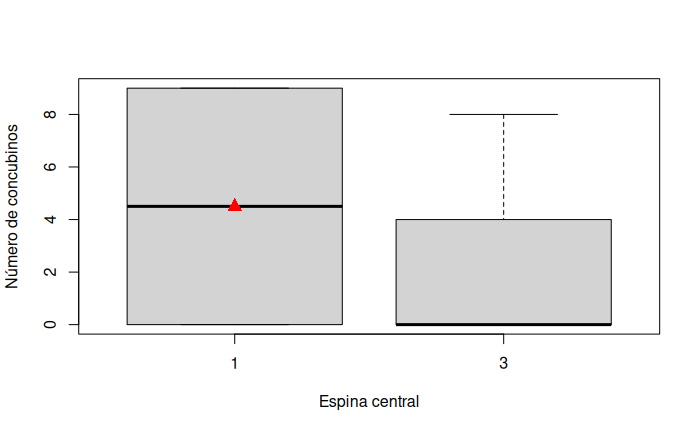
\includegraphics[width=0.7\linewidth]{Images/espina-capa.png}
    \caption{Predicciones por espina.}
    \label{fig:espina-capa}
\end{figure}

%%%%%%%%%%%%%%%%%%%%%%%%%%%%%%%%%%%%%%%%%%%%%%%%%%%%%%%%%%%%%%%%%%%%%%%%%%%
%%%%%%%%%%%%%%%%%%%%%%%%%%%%%%%%%%%%%%%%%%%%%%%%%%%%%%%%%%%%%%%%%%%%%%%%%%%

%%%%%%%%%%%%%%%%%%%%%%%%%%%%%%%%%%%%%%%%%%%%%%%%%%%%%%%%%%%%%%%%%%%%%%%%%%%
%%%%%%%%%%%%%%%%%%%%%%%%%%%%%%%%%%%%%%%%%%%%%%%%%%%%%%%%%%%%%%%%%%%%%%%%%%%

\subsection{Codigo}

\begin{lstlisting}[caption={Modelos de Regresion de Poisson para Cangrejos Cacerola}, label={lst:glm_crabs}]
# Carga y preparacion de datos
crabs <- data.frame(
  Color     = c(3,4,2,4,4,3,2),
  Spine     = c(3,3,1,3,3,3,1),
  Width     = c(28.3,22.5,26.0,24.8,26.0,23.8,26.5),
  Satellite = c(8,0,9,0,4,0,0),
  Weight    = c(3050,1550,2300,2100,2600,2100,2350)
)
crabs$Color <- factor(crabs$Color)
crabs$Spine <- factor(crabs$Spine)

# Funcion auxiliar para calcular IRR (Incidence Rate Ratios)
get_IRR <- function(model){
  ci <- confint.default(model)
  exp(cbind(Estimate = coef(model), ci))
}

# 1) Modelo con Width
m_width <- glm(Satellite ~ Width, data = crabs, family = poisson)
get_IRR(m_width)
newd_w <- data.frame(Width = seq(min(crabs$Width), max(crabs$Width), length.out = 100))
newd_w$mu_hat <- predict(m_width, newdata = newd_w, type="response")
plot(Satellite ~ Width, data = crabs, pch=19,
     xlab="Anchura del caparazon", ylab="Numero de concubinos")
lines(newd_w$Width, newd_w$mu_hat, col="blue", lwd=2)

# 2) Modelo con Weight
m_weight <- glm(Satellite ~ Weight, data = crabs, family = poisson)
get_IRR(m_weight)
newd_wt <- data.frame(Weight = seq(min(crabs$Weight), max(crabs$Weight), length.out = 100))
newd_wt$mu_hat <- predict(m_weight, newdata = newd_wt, type="response")
plot(Satellite ~ Weight, data = crabs, pch=19,
     xlab="Peso", ylab="Numero de concubinos")
lines(newd_wt$Weight, newd_wt$mu_hat, col="blue", lwd=2)
\end{lstlisting}

\subsection{Resumen de codigo}

\begin{itemize}
    \item \textbf{Datos:} Se cargan los datos de los cangrejos en un \texttt{data.frame}. Las variables \texttt{Color} y \texttt{Spine} se convierten a factores para su correcto tratamiento en los modelos.

    \item \textbf{Modelos:} Se ajustan múltiples modelos lineales generalizados univariados con \texttt{glm}, utilizando la familia \texttt{poisson} con enlace logarítmico, que es adecuado para datos de conteo. Cada modelo evalúa la relación entre el número de concubinos (\texttt{Satellite}) y una única variable predictora (ej. \texttt{Width}, \texttt{Weight}).

    \item \textbf{Análisis:} Se define una función auxiliar, \texttt{get\_IRR}, para calcular los \textit{Incidence Rate Ratios} (IRR) y sus intervalos de confianza. Estos valores se utilizan para interpretar el efecto multiplicativo de cada predictor sobre el número esperado de concubinos.

    \item \textbf{Predicciones:} Para las variables continuas (\texttt{Width}, \texttt{Weight}), se generan predicciones del número esperado de concubinos sobre una secuencia de valores, permitiendo trazar una curva de ajuste suave.

    \item \textbf{Visualización:} Se crea un gráfico para cada modelo, mostrando los datos observados (puntos) y la relación predicha por el modelo (línea o puntos de predicción). Esto permite una comparación visual del ajuste del modelo a los datos.
\end{itemize}

\clearpage









